\section{Service Architecture}
\label{sec:architecture}

\subsection{Domain and Motivation}

The platform models a Smart City Environmental Monitoring system serving a mid-sized
Portuguese city. The city is divided into three geographic zones: North (40.671°N, 8.627°W),
Centre (40.641°N, 8.654°W), and South (40.610°N, 8.681°W). Each zone has
IoT sensors reporting air quality (AQI), temperature (°C), and noise levels (dB). Each zone's sensors report
to a Zone Aggregator edge service, which computes per-interval statistics
(average, minimum, maximum) and sends a single batched payload to the central ingestion
service every 10 seconds. This aggregation pattern reduces upstream bandwidth by a factor
equal to the number of sensors per zone, limiting the volume of data
transmitted to the central platform.

\subsection{System Components}

\begin{figure*}[t]
  \centering
  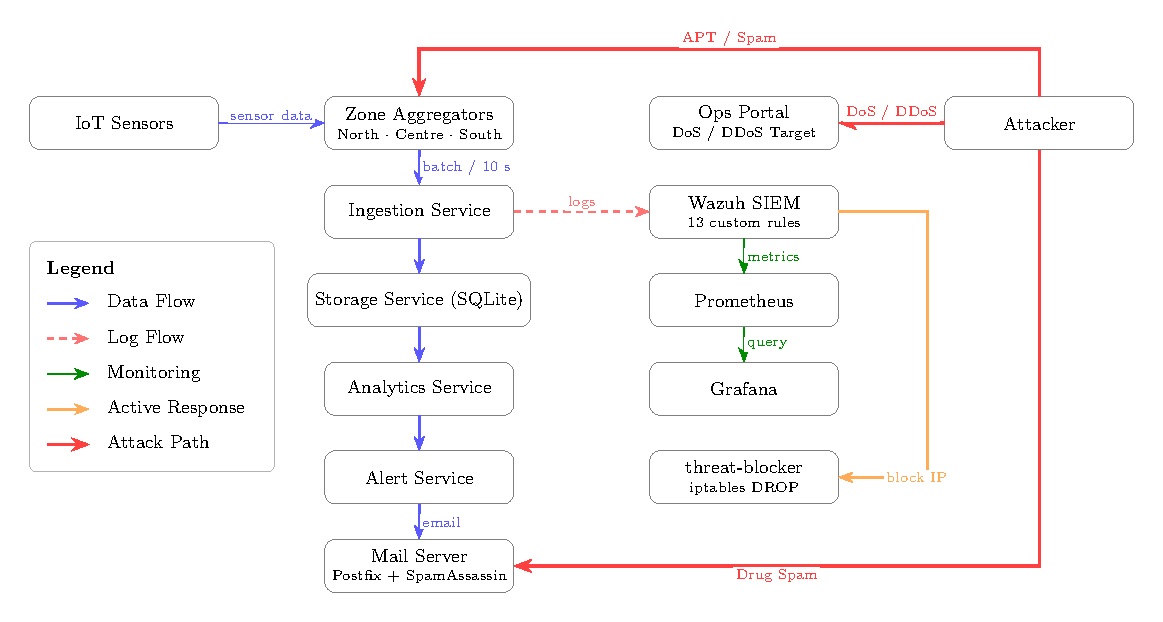
\includegraphics[width=\textwidth]{images/architecture.pdf}
  \caption{Smart City SOA infrastructure.}
  \label{fig:architecture}
\end{figure*}

Figure~\ref{fig:architecture} illustrates the full infrastructure, including data flows,
observability paths, and active response chain. Three zone aggregator services operate
on ports 5100, 5101, and 5102 for the
North, Centre, and South zones respectively. Each aggregator spawns three sensor
simulation threads, collects readings into a buffer, and forwards aggregated payloads
to the ingestion service. Access logs are written as structured JSON to a shared
volume mounted by Wazuh. Intentional honeypot endpoints (\texttt{/api/admin/config}
and \texttt{/api/admin/metrics}) are exposed to simulate a misconfigured debug
interface that leaks the \texttt{INTERNAL\_TOKEN} (the shared secret used to
authenticate inter-service calls).

The central platform comprises six services:

\begin{itemize}[leftmargin=*]
  \item \textbf{Service registry} (port 5050) - zone-aware service discovery with
        geographic metadata. Services register on startup and send heartbeats every 30 seconds.
  \item \textbf{Ingestion service} (port 5200) - receives zone payloads, validates
        data ranges, and forwards to storage.
  \item \textbf{Storage service} - SQLite-backed persistence of time-series readings.
  \item \textbf{Analytics service} - Aggregation queries and zone statistics.
  \item \textbf{Alert service} (port 5500) - monitors thresholds and sends email
        alerts when sensor readings exceed configured limits. A circuit breaker enforces
        a 5 minute cooldown after 12 consecutive emails, and Postfix applies a hard
        rate limit of 30 messages per minute.
  \item \textbf{Ops portal} (port 5600) - web dashboard for city operators and the
        primary target of DoS and DDoS attacks.
\end{itemize}

The mail server runs Postfix 3.6 with SpamAssassin content filtering on port 25.
A custom Python exporter exposes Prometheus metrics on port 9154 by tailing
Postfix logs.

The monitoring stack comprises four components: Prometheus (port 9090) scrapes all
services at a 15-second interval; Grafana (port 3000) provides the security
dashboard; the Wazuh exporter (port 9100) bridges Wazuh to Prometheus by tailing
\texttt{alerts.json} and polling the Wazuh REST API; and the threat-blocker service
(port 9200) receives block requests from Wazuh's active response script and applies
\texttt{iptables} DROP rules in the \texttt{DOCKER-USER} chain, with automatic
unblock after 300 seconds.

\subsection{Communication and Data Flow}

Inter-service calls are authenticated via a shared token distributed through the
\texttt{x-internal-token} HTTP header, generated at deploy time and distributed via
an environment file. All services write structured JSON access logs (including
timestamp, client IP, method, path, event type, and zone) to a shared Incus
bind-mount, which Wazuh ingests in real time.

\subsection{Security Mechanisms}

\begin{itemize}[leftmargin=*]
  \item \textbf{Internal token authentication:} as described above, all inter-service
        calls require the shared token. Requests that fail this check are logged as
        \texttt{auth\_failed} events, triggering Wazuh rules 100100 and 100101.
  \item \textbf{Honeypot endpoints:} \texttt{/api/admin/config} and
        \texttt{/api/admin/metrics} on zone aggregators log every access as a
        \texttt{HONEYPOT\_HIT} event. There is no legitimate caller for these paths.
  \item \textbf{404 logging:} a FastAPI exception handler logs all requests to unknown
        paths as \texttt{not\_found} events, enabling recon phase detection.
  \item \textbf{IP-level blocking:} \texttt{threat-blocker} writes DROP rules to
        \texttt{DOCKER-USER} rather than the \texttt{INPUT} chain, correctly intercepting
        traffic that is DNAT-forwarded by Docker before it reaches service processes.
\end{itemize}

\subsection{Infrastructure and Deployment Rationale}

The platform runs inside a Debian 13 VirtualBox VM (8 GB RAM, 6 CPUs). Available disk space on the host constrained all
components to this single VM, which already had Incus installed with a running Wazuh
instance. Two isolation layers are therefore used: Incus system containers for
host-level isolation, and Docker Compose inside one of those containers for the SOA
services.

Docker Compose was chosen as a second layer because the SOA comprises fourteen
interdependent services that require a shared internal network with stable DNS
resolution between them.

Log sharing between the two isolation layers is achieved through two host-level
bind-mounts: one exposes the Docker service logs to Wazuh for real-time ingestion,
and one exposes the Wazuh alert output to the Docker stack for the Wazuh exporter
to read.
